\documentclass[]{article}

\usepackage[utf8]{inputenc}
\usepackage{amsmath}
\usepackage{amssymb}
\usepackage{amsthm}
\usepackage{amsfonts}
\usepackage{graphicx}
\usepackage{capt-of}
\usepackage{listings}
\usepackage{siunitx}
\usepackage{float}
\usepackage[section]{placeins}



% Oppgavenummerering %
\renewcommand\thesection{Task \arabic{section}}
\renewcommand\thesubsection{\alph{subsection})}

% Bevis
\newcommand\TombStone{\rule{.5em}{.5em}}
\renewcommand\qedsymbol{\TombStone}
\renewcommand{\proofname}{Bevis.} % Norske bevis

\title{TDT4195 – IP Assignment 3}
\author{Sigurd Totland | MTTK}

\begin{document}
\maketitle

\section{Theory}
\subsection{}
Opening is dilation of the erotion, i.e. $(A \ominus B) \oplus B$, whereas closing is the erosion of the dilation, i.e. $(A \oplus B) \ominus B$. The typical interpretation of these operations is that closing fills small holes in the image (removes small black objects) and opening removes small (white) objects.

\subsection{}
Edge detection algorithms typically use small kernels, which will pick up both large and tiny edges. Such tiny edges are often found all over an image and are typically caused by noise, texture and other features that we would normally not consider "real edges". To surpress these edges from appearing in the output, but still keep the dominant edges of the image, we can apply smoothing beforehand. The choice of blur comes down to choice of how detailed we want the edge detection to be. With little or no blur, all edges will be picked up, whereas with lots of blur, only dominant edges will show.

\subsection{}
Hysterisis thresholding is a type of adaptive thresholding where pixels are regarded as above the threshold if they are neighbor to some high-valued pixel. For this, the algorithm typically has two threshold levels, one higher and one lower. And a pixel can be considered above the threshold if it is at least above the lower threshold and it neighbors some pixel above the higher threshold.
\begin{figure}[H]
\centering
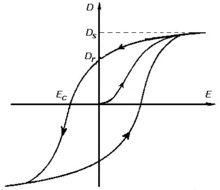
\includegraphics[width=0.45\textwidth]{hysterisis}
\caption{Hysterisis. Neighboring a bright pixel can be thought of as traversing the left-going curve, which will require a lower intensity to be regarded as above the threshold than when traversing the right-going curve.}
\label{fig:hysterisis}
\end{figure}

\subsection{}
The Canny edge detector uses hysterisis thresholding after edge detection instead of regular thresholding because it is better at connecting edges and removing noise that is not clearly part of an edge. The example image in figure \ref{fig:hysterisis_skimage} below from the \texttt{skimage} docs shows how hysterisis thresholding, when applied after a sobel edge detection filter preserves edges and removes unwanted noise much better than regular thresholding.

\begin{figure}[H]
\centering
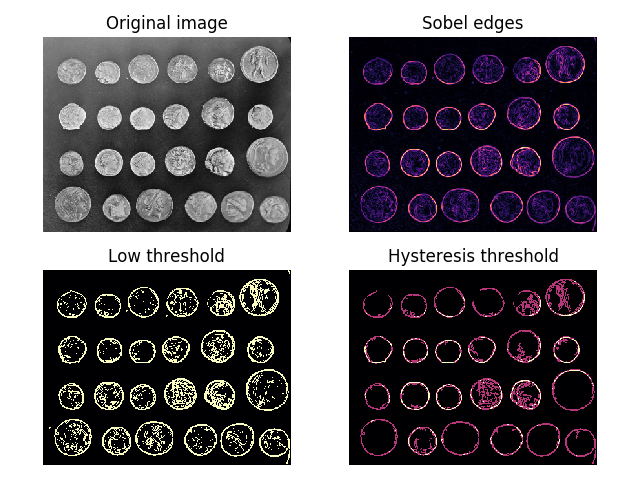
\includegraphics[width=0.8\textwidth]{hysterisis_skimage}
\caption{Hysterisis thresholding vs regular thresholding}
\label{fig:hysterisis_skimage}
\end{figure}

\subsection{}
\begin{equation}\begin{aligned}
\begin{bmatrix}
0 & 0 & 0 & 0 & 0 & 0 \\
1 & 0 & 0 & 0 & 1 & 0 \\
0 & 1 & 1 & 1 & 0 & 0 \\
1 & 0 & 0 & 0 & 1 & 0 \\
0 & 0 & 1 & 0 & 0 & 0 \\
0 & 0 & 0 & 0 & 0 & 0 \\
\end{bmatrix}
\oplus
\begin{bmatrix} 1 & 1 & 1 \end{bmatrix} =
\begin{bmatrix}
0 & 0 & 0 & 0 & 0 & 0 \\
1 & 1 & 0 & 1 & 1 & 1 \\
1 & 1 & 1 & 1 & 1 & 0 \\
1 & 1 & 0 & 1 & 1 & 1 \\
0 & 1 & 1 & 1 & 0 & 0 \\
0 & 0 & 0 & 0 & 0 & 0 \\
\end{bmatrix}
\end{aligned}\end{equation}

\end{document}

